\documentclass[lettersize,journal]{ieee_template/IEEEtran}
\usepackage{amsmath,amsfonts}
\usepackage{array}
\usepackage{booktabs}
\usepackage{graphicx}
\usepackage{url}
\usepackage{cite}
\usepackage{tikz}
\usetikzlibrary{arrows.meta,positioning,shapes.geometric,fit}

\begin{document}

\title{Virtuoso-Bridge: An Agent-Native Bridge for Remote and Programmable Cadence Virtuoso Workflows}

\author{Zhishuai~Zhang, Xintian~Li, Nan~Sun, Lu~Jie%
\thanks{All authors are with Tsinghua University.}%
}

\markboth{}%
{Zhang: Virtuoso-Bridge}

\maketitle

\begin{abstract}
Agent-driven analog and mixed-signal (AMS) workflows require a stable and agent-native software boundary between Python code and the Cadence Virtuoso environment. This paper presents Virtuoso-Bridge, an open-source bridge that encapsulates the standard SKILL IPC mechanism, namely \texttt{ipcBeginProcess} and \texttt{evalstring}, as a practical implementation for local and remote use. The system separates SKILL execution (VirtuosoClient) from transport and deployment (SSHClient), allowing the same client code to operate in local, LAN, VPN, and multi-hop SSH environments. On top of this boundary, Virtuoso-Bridge provides raw SKILL execution, SKILL script injection, and Python APIs for layout, schematic, and Spectre-related workflows. The repository further includes agent-native workflow support through CLI lifecycle management, persistent tunnels, structured skill files, screenshot-based verification, and runnable examples spanning layout, schematic, ADE Assembler (Maestro), and Spectre tasks. This report characterizes the resulting agent-native tooling boundary and documents the workflow scope currently supported by the tool.
\end{abstract}

\begin{IEEEkeywords}
Cadence Virtuoso, agent-native tooling, Python automation, remote access, SSH tunneling, analog IC design, EDA workflows.
\end{IEEEkeywords}

%═══════════════════════════════════════════════════════════════════════
\section{Introduction}
%═══════════════════════════════════════════════════════════════════════
\IEEEPARstart{T}{he} core mechanism for programmatic access to Cadence Virtuoso is well established. The SKILL language provides \texttt{ipcBeginProcess}, which spawns a child process inside the Virtuoso runtime and connects it through stdin/stdout pipes. The child process receives SKILL expressions, and Virtuoso evaluates them via \texttt{evalstring}. Results flow back through the same pipe.

SkillBridge~\cite{skillbridge} and Virtuoso-Bridge both build on this same IPC pattern, in which a child process receives SKILL expressions and returns evaluated results through the Virtuoso IPC channel.

The key design consideration is therefore not the execution mechanism itself, since that mechanism already exists, but the system boundary built around it. SkillBridge answers this question with a transparent Pythonic RPC layer in which Python objects map to SKILL objects, function calls map to SKILL calls, and the user interacts as if writing SKILL in Python syntax. This model provides effective support for interactive local exploration.

By contrast, Virtuoso-Bridge adopts an agent-native execution boundary that packages bridge lifecycle, remote transport, editing operations, and artifact return into a single project-local system. The resulting tool emphasizes four practical properties: transparent remote access through SSH tunnels, multiple programming levels from raw SKILL to Python APIs, feedback channels for visual and numerical checking, and lifecycle support for repeated agent use.

This work was motivated by our experience building AMS-IO-Agent~\cite{amsioagent}, an LLM-based agent for I/O ring design that was validated in a CMOS tape-out. In that project, the lack of a stable, remote-capable, and agent-friendly bridge between the agent and Virtuoso emerged as a central infrastructure requirement. Virtuoso-Bridge is the distilled and generalized result of that effort. The goal of this paper is to report the design, scope, and practical usage model of the resulting tool rather than to introduce a new execution primitive.

%═══════════════════════════════════════════════════════════════════════
\section{Design and Architecture}
%═══════════════════════════════════════════════════════════════════════

The central design choice is the separation of \emph{what to execute} from \emph{how to reach the execution environment}. This is realized through two independent modules.

\begin{figure*}[!t]
\centering
\resizebox{\textwidth}{!}{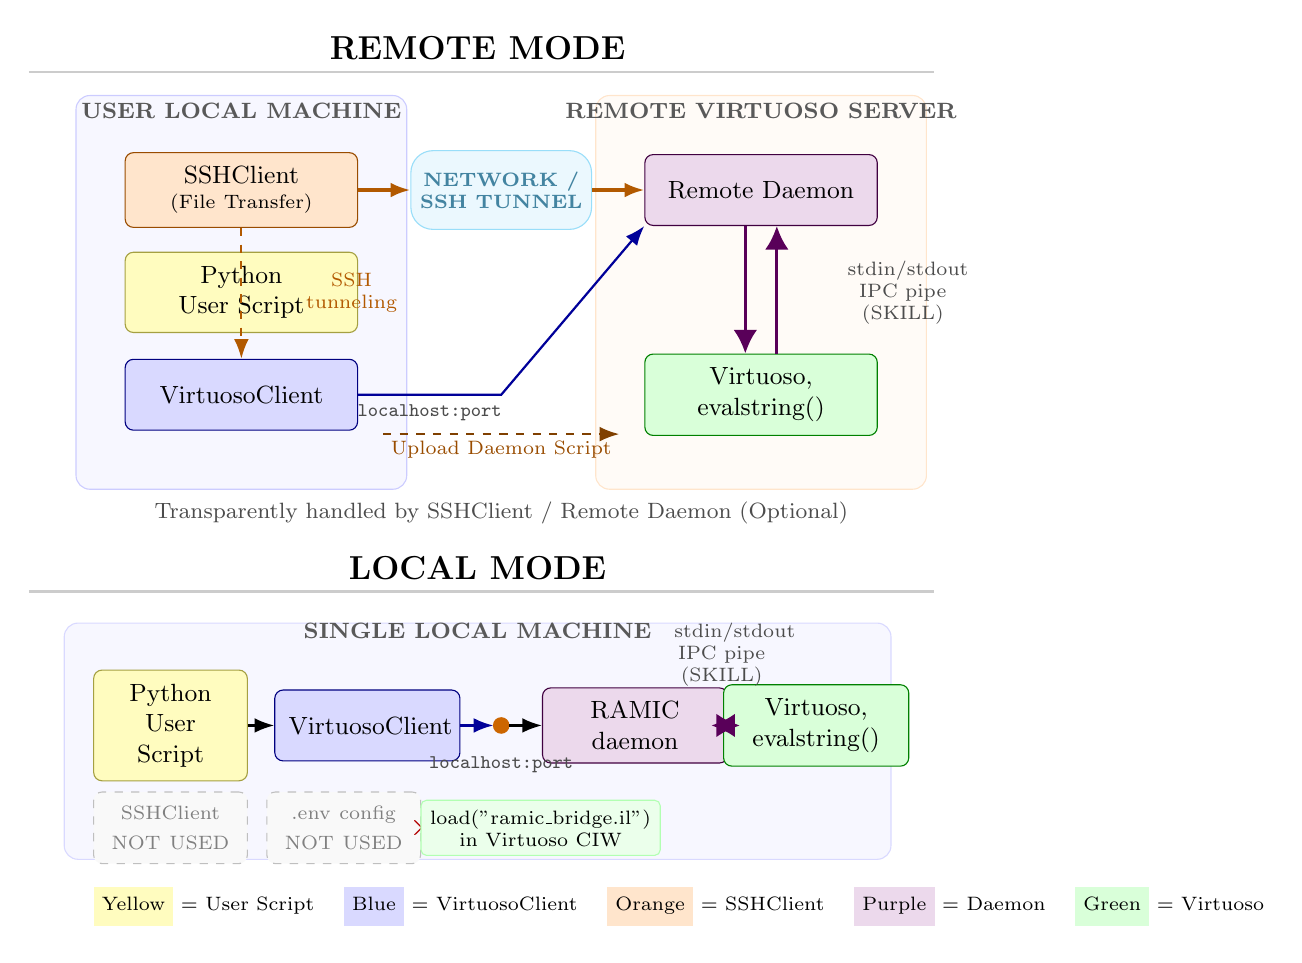
\begin{tikzpicture}[
  font=\small,
  box/.style={draw, rounded corners=3pt, minimum height=0.9cm, inner sep=5pt, align=center, text width=2.6cm},
  userbox/.style={box, fill=yellow!25, draw=yellow!60!black},
  clientbox/.style={box, fill=blue!15, draw=blue!50!black},
  sshbox/.style={box, fill=orange!20, draw=orange!60!black},
  daemonbox/.style={box, fill=violet!15, draw=violet!50!black},
  virtbox/.style={box, fill=green!15, draw=green!50!black},
  graybox/.style={box, draw=gray!50, fill=gray!5, dashed, text=gray, text width=1.6cm, minimum height=0.7cm},
  region/.style={draw, rounded corners=5pt, inner sep=10pt},
  localregion/.style={region, fill=blue!3, draw=blue!20},
  remoteregion/.style={region, fill=orange!3, draw=orange!20},
  singleregion/.style={region, fill=blue!3, draw=blue!15},
  modetitle/.style={font=\bfseries\large},
  sectiontitle/.style={font=\footnotesize\bfseries, text=gray!70!black},
  arr/.style={-{Latex[length=2.5mm]}, thick},
  darr/.style={-{Latex[length=2.5mm]}, thick, dashed},
  bigarr/.style={-{Latex[length=3mm,width=3mm]}, very thick, violet!70!black},
  note/.style={font=\scriptsize, text=gray!60!black, align=center},
]

% ====== REMOTE MODE ======
\node[modetitle] at (4.2, 9.6) {REMOTE MODE};
\draw[thick, gray!40] (-1.5, 9.3) -- (10.0, 9.3);

% Local machine region
\node[localregion, minimum width=4.2cm, minimum height=5.0cm] (localbox) at (1.2, 6.5) {};
\node[sectiontitle] at (1.2, 8.8) {USER LOCAL MACHINE};

% Remote server region
\node[remoteregion, minimum width=4.2cm, minimum height=5.0cm] (remotebox) at (7.8, 6.5) {};
\node[sectiontitle] at (7.8, 8.8) {REMOTE VIRTUOSO SERVER};

% Local components
\node[sshbox] (ssh) at (1.2, 7.8) {SSHClient\\[-2pt]{\scriptsize (File Transfer)}};
\node[userbox] (user) at (1.2, 6.5) {Python\\User Script};
\node[clientbox] (vc) at (1.2, 5.2) {VirtuosoClient};

% Remote components
\node[daemonbox] (daemon) at (7.8, 7.8) {Remote Daemon};
\node[virtbox] (virt) at (7.8, 5.2) {Virtuoso,\\evalstring()};

% SSH tunnel cloud
\node[draw, rounded corners=8pt, fill=cyan!8, draw=cyan!40, minimum width=1.8cm, minimum height=1.0cm, align=center, font=\scriptsize\bfseries, text=cyan!60!black] (cloud) at (4.5, 7.8) {NETWORK /\\SSH TUNNEL};

% Arrows - SSH path (file transfer + tunnel)
\draw[arr, orange!70!black, very thick] (ssh.east) -- (cloud.west);
\draw[arr, orange!70!black, very thick] (cloud.east) -- (daemon.west);

% Dashed line SSH tunneling label
\draw[darr, orange!70!black] (ssh.south) -- (vc.north);
\node[note, text=orange!70!black] at (2.6, 6.5) {SSH\\tunneling};

% Arrow - TCP data flow (VirtuosoClient to daemon via tunnel)
\draw[arr, blue!60!black] (vc.east) -- node[below, note] {\texttt{localhost:port}} (4.5, 5.2) -- (daemon.south west);

% Arrow - IPC pipe (bidirectional)
\draw[bigarr] ([xshift=-2mm]daemon.south) -- ([xshift=-2mm]virt.north);
\draw[bigarr] ([xshift=2mm]virt.north) -- ([xshift=2mm]daemon.south);
\node[note, text width=1.4cm] at (9.6, 6.5) {stdin/stdout\\IPC pipe\\(SKILL)};

% Upload daemon label
\node[note, text=orange!60!black] at (4.5, 4.5) {Upload Daemon Script};
\draw[darr, orange!50!black] (3.0, 4.7) -- (6.0, 4.7);

% Bottom label
\node[note, font=\footnotesize] at (4.5, 3.7) {Transparently handled by SSHClient / Remote Daemon (Optional)};

% ====== LOCAL MODE ======
\node[modetitle] at (4.2, 3.0) {LOCAL MODE};
\draw[thick, gray!40] (-1.5, 2.7) -- (10.0, 2.7);

% Single machine region
\node[singleregion, minimum width=10.5cm, minimum height=3.0cm] at (4.2, 0.8) {};
\node[sectiontitle] at (4.2, 2.2) {SINGLE LOCAL MACHINE};

% Local mode components
\node[userbox, text width=1.6cm] (luser) at (0.3, 1.0) {Python\\User Script};
\node[clientbox, text width=2.0cm] (lvc) at (2.8, 1.0) {VirtuosoClient};
\node[daemonbox, text width=2.0cm] (ldaemon) at (6.2, 1.0) {RAMIC daemon};
\node[virtbox, text width=2.0cm] (lvirt) at (8.5, 1.0) {Virtuoso,\\evalstring()};

% Arrows
\draw[arr] (luser.east) -- (lvc.west);

% Orange dot for localhost:port
\fill[orange!80!black] (4.5, 1.0) circle (3pt);
\draw[arr, blue!60!black] (lvc.east) -- (4.4, 1.0);
\draw[arr] (4.6, 1.0) -- (ldaemon.west);
\node[note] at (4.5, 0.5) {\texttt{localhost:port}};

% IPC arrows
\draw[bigarr] ([xshift=-1.5mm]ldaemon.east) -- ([xshift=-1.5mm]lvirt.west);
\draw[bigarr] ([xshift=1.5mm]lvirt.west) -- ([xshift=1.5mm]ldaemon.east);
\node[note, text width=1.2cm] at (7.3, 1.9) {stdin/stdout\\IPC pipe\\(SKILL)};

% Not used labels
\node[graybox] at (0.3, -0.3) {\scriptsize SSHClient\\NOT USED};
\node[graybox] at (2.5, -0.3) {\scriptsize .env config\\NOT USED};
\node[font=\large, text=red!70!black] at (3.5, -0.3) {\texttimes};

% load label
\node[draw, rounded corners=2pt, fill=green!8, draw=green!30, font=\scriptsize, align=center] at (5.0, -0.3) {load("ramic\_bridge.il")\\in Virtuoso CIW};

% ====== COLOR LEGEND ======
\node[font=\scriptsize, anchor=west] at (-0.8, -1.3) {%
\colorbox{yellow!25}{\strut Yellow} = User Script \quad
\colorbox{blue!15}{\strut Blue} = VirtuosoClient \quad
\colorbox{orange!20}{\strut Orange} = SSHClient \quad
\colorbox{violet!15}{\strut Purple} = Daemon \quad
\colorbox{green!15}{\strut Green} = Virtuoso};

\end{tikzpicture}
}
\caption{Decoupled architecture showing both remote and local modes. In remote mode, SSHClient creates an SSH tunnel and deploys the daemon. VirtuosoClient connects to a TCP endpoint without knowing whether it is local or tunneled. In local mode, SSHClient is not used.}
\label{fig:architecture}
\end{figure*}

\textbf{VirtuosoClient} is a pure TCP client. It connects to \texttt{localhost:port}, sends SKILL code as a JSON payload, and receives results with binary framing using STX/NAK delimiters. It is agnostic to SSH, remote hosts, and file transfer. User Python code calls VirtuosoClient first; when a tunnel is attached, file upload, download, and \texttt{load\_il()} preparation delegate to SSHClient, while SKILL execution still goes only through the TCP daemon endpoint.

\textbf{SSHClient} is a tunnel and deployment manager. In remote mode it establishes an SSH port forward, uploads the daemon and setup files, and manages file transfer. In local mode it is absent: the user loads the local IL file in the Virtuoso CIW, and \texttt{VirtuosoClient.local()} connects directly to the local daemon.

This decoupling allows VirtuosoClient to be tested without SSH infrastructure, and changing the transport from SSH to VPN or direct LAN requires no client code changes. The tunnel process is detached and survives across Python script invocations, and port conflicts are resolved automatically by trying successive ports and writing the working port back to the configuration file.

The communication protocol between VirtuosoClient and the daemon is deliberately simple. The client opens one TCP connection per request and sends a JSON object containing the SKILL string and a timeout value. The daemon passes the SKILL string to Virtuoso via \texttt{evalstring}, then returns the result with binary framing: \texttt{0x02} (STX) for success, \texttt{0x15} (NAK) for error, and \texttt{0x1E} (RS) as terminator. Because Virtuoso is single-threaded, the daemon also handles requests serially. Additional requests wait at the TCP accept/connect boundary rather than being executed in parallel or intentionally dropped.

The \texttt{core/} directory of the repository contains the entire bridge mechanism in 3 files totaling 180 lines.

%═══════════════════════════════════════════════════════════════════════
\section{API Levels}
%═══════════════════════════════════════════════════════════════════════

A single interaction granularity is insufficient for AMS workflows. Virtuoso-Bridge provides three levels, and an agent can switch among them as needed.

\subsection{Level 1: Raw SKILL Execution}
The method \texttt{client.execute\_skill()} sends an arbitrary SKILL expression to Virtuoso and returns the result, equivalent to typing in the CIW console.

\noindent{\ttfamily\small
client.execute\_skill('printf("Hello!")')\\
client.execute\_skill("getVersion()")\\
client.execute\_skill("getHostName()")\par}

Batch execution via \texttt{execute\_operations} reduces round-trip overhead.

\subsection{Level 2: Script Injection}
The method \texttt{client.load\_il()} uploads a SKILL file to the remote host and loads it into the running Virtuoso session. This level is suitable for encapsulated operations packaged once in reusable helper IL files.

\noindent{\ttfamily\small
client.load\_il("list\_library\_cells.il")\\
client.load\_il("screenshot.il")\par}

\subsection{Level 3: Pythonic APIs}
Context-managed editors abstract common schematic and layout patterns.

Schematic example:

\noindent{\ttfamily\small
with client.schematic.edit(lib, cell) as sch:\\
sch.add\_instance("analogLib", "res", (0.0, 0.0), name="R0")\\
sch.add\_wire([(0.0, 0.0), (1.2, 0.0)])\\
sch.add\_pin("OUT", "output", (1.2, 0.0))\par}

Layout example:

\noindent{\ttfamily\small
with client.layout.edit(lib, cell) as ly:\\
ly.add\_rect("M1", "drawing", (1.0, 0.0, 2.0, 0.5))\\
ly.add\_path("M2", "drawing", [(1.0, 0.25), (2.5, 0.25)], width=0.1)\\
ly.add\_via("M1\_M2", (1.5, 0.25))\par}

The editor translates these calls into SKILL and handles open/save/close automatically. Representative schematic examples include stepwise RC-filter construction and terminal-aware net labeling, while layout examples include scripted rectangle or via insertion. This level is most suitable for AI agents because it reduces the amount of SKILL syntax they must generate directly.

\input{tables/comparison.tex}

%═══════════════════════════════════════════════════════════════════════
\section{Feedback Channels}
%═══════════════════════════════════════════════════════════════════════

An agent operating in an EDA environment cannot rely solely on textual return values. Layout correctness, schematic topology, and waveform shapes are inherently visual. Virtuoso-Bridge provides several multimodal return paths to address this limitation.

\paragraph{Screenshot-based visual verification.} The repository includes a screenshot workflow based on a small SKILL helper script together with file transfer through the bridge. This allows the current Virtuoso window to be captured, transferred to the local machine, and returned to the agent. When combined with a vision-language model (VLM), the agent can inspect the resulting image and decide whether a layout or schematic edit is correct before proceeding.

\paragraph{Simulation data.} Spectre simulation results are parsed from PSF ASCII format into Python data structures, supporting both real-valued (transient, DC) and complex-valued (AC) waveforms. The agent can inspect waveform data programmatically, compute derived metrics such as capacitance from AC current or the $f_\mathrm{3dB}$ from a frequency response, and make optimization decisions without manual intervention.

\paragraph{File transfer.} Arbitrary files can be uploaded to or downloaded from the remote Virtuoso host through the SSH tunnel. This supports workflows such as netlist export, result archival, and exchange of intermediate artifacts between agent rounds.

\paragraph{Command logging.} All SSH and SKILL commands are logged with timestamps to a persistent log file. This provides full traceability for debugging agent-driven workflows and enables post-hoc analysis of agent behavior.

These return paths collectively enable closed-loop iteration, in which the agent issues a command, observes the result through the appropriate modality, reasons about whether the outcome is correct, and corrects if necessary.

%═══════════════════════════════════════════════════════════════════════
\section{Agent-Native Features}
%═══════════════════════════════════════════════════════════════════════

An agent-native system differs from a conventional API in that it must support autonomous, repeated tool use without human setup at each round. Virtuoso-Bridge addresses this requirement through several design choices.

\paragraph{CLI-first lifecycle.} After the one-time Virtuoso-side setup step, the bridge lifecycle is managed through the commands \texttt{virtuoso-bridge start}, \texttt{status}, \texttt{restart}, and \texttt{stop}. Agents invoke these commands without repeated GUI interaction. The \texttt{status} command reports tunnel health, daemon responsiveness, remote hostname verification, and, when configured, Spectre license availability in a single call.

\paragraph{Skill files.} The \texttt{skills/} directory contains structured documents covering the virtuoso, spectre, and optimizer workflows. An agent reads the relevant skill file and obtains task-oriented guidance on which APIs to call, what the workflow looks like, and what pitfalls to avoid. This reduces the amount of ad hoc prompt scaffolding required from the user.

\paragraph{Persistent tunnel.} The SSH tunnel process is detached from the parent Python process and survives across script invocations. Tunnel state, including PID, port, and remote host, is persisted to a JSON file and reused by subsequent connections. This eliminates the repeated setup cost that would otherwise dominate high-frequency agent interaction. On Windows, platform-specific process detachment flags are used to ensure tunnel stability.

\paragraph{Runnable examples.} The repository includes over 30 runnable examples covering layout editing, schematic creation, CDL netlist import via \texttt{spiceIn}, Spectre netlist export via ADE Assembler (Maestro) SKILL APIs, ADE Assembler (Maestro) test creation with parametric sweeps and spec checking, and Spectre simulation including transient, DC+AC, and PSS+Pnoise analyses. These serve as both documentation and few-shot references for agents. Most examples require only \texttt{analogLib} and run without a specific PDK.

%═══════════════════════════════════════════════════════════════════════
\section{Simulation Integration}
%═══════════════════════════════════════════════════════════════════════

Spectre simulation is integrated as a first-class capability.

\noindent{\ttfamily\small
sim = SpectreSimulator.from\_env(\\
\hspace*{1em}work\_dir="./out")\\
result = sim.run\_simulation("tb.scs", \{\})\par}

The system automatically sources the Cadence environment on the remote host, uploads netlists and include files including Verilog-A modules, executes Spectre, downloads PSF results, and parses them into Python data structures. Multiple simulation modes are supported, including basic Spectre, APS, and Spectre~X.

When the Cadence environment configuration is provided, license availability is checked via the \texttt{status} command, which queries \texttt{lmstat} on the remote host and reports feature usage. This helps prevent agents from submitting simulations that would wait indefinitely for unavailable licenses, a failure mode that is otherwise difficult to diagnose.

%═══════════════════════════════════════════════════════════════════════
\section{Relation to SkillBridge}
%═══════════════════════════════════════════════════════════════════════

Table~\ref{tab:comparison_ieee} summarizes the positioning of Virtuoso-Bridge relative to SkillBridge.

Both systems use the same three SKILL calls, namely \texttt{ipcBeginProcess}, \texttt{evalstring}, and \texttt{ipcWriteProcess}. The SKILL-side code differs mainly in response framing, with one using binary delimiters and the other using text prefixes. The main difference lies in what is built on top of this shared foundation.

SkillBridge provides transparent Python-to-SKILL type mapping, IDE tab completion, and an interactive programming model optimized for human exploration.

Virtuoso-Bridge provides SSH remote access, script injection, structured layout and schematic APIs, CDL netlist import (\texttt{spiceIn}), Spectre netlist export, ADE Assembler (Maestro) control for simulation setup and result analysis, standalone Spectre simulation integration, multimodal feedback, and agent-native lifecycle management. These capabilities are designed for automated, remote, high-frequency workflows driven by coding agents.

%═══════════════════════════════════════════════════════════════════════
\section{Scope of Supported Workflows}
%═══════════════════════════════════════════════════════════════════════

This paper is intended as a tool report, so the emphasis is on the supported scope of the bridge and the workflows exercised with it.

\paragraph{Execution modes.} The bridge supports both remote operation through SSH, including jump-host configurations, and local operation without SSH. The same VirtuosoClient interface is used in both modes, while SSHClient remains optional in local deployments.

\paragraph{Workflow coverage.} The open-source repository includes runnable examples for raw SKILL execution, loading and calling external \texttt{.il} files, layout editing, schematic editing, screenshot-based visual checking, CDL import via \texttt{spiceIn}, ADE Assembler (Maestro) control through \texttt{mae*} SKILL APIs, and Spectre simulation flows including transient, DC+AC, and PSS+Pnoise analyses.

\paragraph{Platform scope.} The open-source package targets macOS, Windows, and Linux, and supports both local and remote workflows from the same repository.

\paragraph{Operational preconditions.} In remote mode, the bridge assumes that SSH access to the target host is already functional and that a Virtuoso process is already running. First-time use still requires a one-time setup action in the Virtuoso CIW to load the generated setup script. In addition, Spectre license checking depends on the Cadence environment being configured on the target machine.

\paragraph{Design boundaries and release scope.} Virtuoso-Bridge does not attempt to replace native Virtuoso SKILL or to provide full Python-to-SKILL object-level bidirectional mapping. The screenshot workflow is implemented through a small helper script together with file transfer rather than through a dedicated built-in image API. The fuller harness from which virtuoso-bridge-lite is distilled was used in the development of AMS-IO-Agent~\cite{amsioagent}, where an LLM-based agent completed I/O ring design tasks that contributed to a silicon tape-out workflow. The open-source release preserves the core bridge and workflow interfaces, but does not reproduce every environment-specific detail from the internal deployment from which it was derived.

%═══════════════════════════════════════════════════════════════════════
\section{Conclusion}
%═══════════════════════════════════════════════════════════════════════

Virtuoso-Bridge does not introduce a new Virtuoso execution mechanism. Instead, it provides a structured encapsulation of the standard SKILL IPC facility through an agent-native tool boundary with decoupled transport and execution layers, three levels of programmability, workflow support for visual verification and simulation, and lifecycle management for repeated agent use.

\begin{thebibliography}{2}

\bibitem{skillbridge}
N.~Buwen and T.~Markus, ``SkillBridge,'' GitHub repository. [Online]. Available: \texttt{https://github.com/unihd-cag/skillbridge}

\bibitem{amsioagent}
Z.~Zhang, X.~Li, S.~Liu, A.~Zhang, L.~Jie, and N.~Sun, ``AMS-IO-Bench and AMS-IO-Agent: Benchmarking and structured reasoning for analog and mixed-signal integrated circuit input/output design,'' in \emph{Proc. AAAI Conference on Artificial Intelligence}, vol.~40, no.~2, pp.~1579--1586, Mar. 2026, doi: 10.1609/aaai.v40i2.37134.


\end{thebibliography}

\end{document}
